\documentclass{beamer}

% Indicate to use hyperlink and in which color put them 
\usepackage{hyperref}
\hypersetup{
    colorlinks=true,
    linkcolor=orange,
    filecolor=magenta,      
    urlcolor=blue,
}

% Define the presentation them
\usetheme{Warsaw}

% Set the general color
\definecolor{Dark-lavender}{rgb}{0.45, 0.31, 0.59}
\usecolortheme[named=Dark-lavender]{structure}

% Define the context element
\title{How to developp with Kubernetes}
\subtitle{Developper worstation's tools}
\author{Damien Ribeiro}
\institute{
\includegraphics[height=0.8cm]{tinkou.pdf}}

% Enable to aligne description
\usepackage{calc}  
\usepackage{enumitem} 
% Add an option to left align element in a description
\defbeamertemplate{description item}{align left}{\insertdescriptionitem\hfill}

% Define table of content depth
\setcounter{tocdepth}{1}

\begin{document}
	\frame {
		\titlepage
	}
	
		
	\frame{
		\frametitle{Outline}
		\tableofcontents
	}
	
	
	\frame {
		\frametitle{Pre-requirements}

		\begin{block}{Skills}
			\begin{itemize}
				\item Be comfortable with UNIX command line
				\item Docker notions
				\item Kubernetes notions
			\end{itemize}
		\end{block}
		
		\begin{block}{Resources}
			\begin{itemize}
				\item A computer or a VM with docker installed
				\item An access to a docker registry
				\item An access to a kubernetes cluster
			\end{itemize}
		\end{block}
		
	}

	
	\begin{frame}
	\frametitle{In local with minikube}
	
	We need to install the tools used during the workshops:
	\begin{description}[leftmargin=!,labelwidth=\widthof{\bfseries Kustomize}]
		\item[Docker] \href{https://hub.docker.com/search/?type=edition&offering=community}{Official release page}
		\item[Kubectl] \href{https://kubernetes.io/docs/tasks/tools/install-kubectl/}{Official installation documentation}
		\item[Minikube] \href{https://kubernetes.io/docs/tasks/tools/install-minikube/}{Official installation documentation}
		\item[Kustomize] \href{https://github.com/kubernetes-sigs/kustomize/blob/master/docs/INSTALL.md}{Official installation documentation}
		\item[Skaffold] \href{https://skaffold.dev/docs/getting-started/\#installing-skaffold}{Official installation documentation}
		\item[Stern] \href{https://github.com/wercker/stern}{Official installation documentation}
	\end{description}	
\end{frame}

\begin{frame}[fragile]
	\frametitle{In local with minikube}
	
	Minikube consist of a single node kubernetes cluster. Here a few commands usefull for the workshop:
	
	\begin{block}{Get the cluster IP. This IP will be used as the one of each kubernetes servers (master or node):}
		\begin{verbatim}
			minikube ip
		\end{verbatim}
	\end{block}
	
	\medskip	
	
	\begin{block}{Use the docker daemon of minikube instead of a local one:}
		\begin{verbatim}
			eval $(minikube docker-env)
		\end{verbatim}
	\end{block}
	
	\medskip
	For the registry, we will use the docker local registry of minikube.
\end{frame}
	
	\begin{frame}[fragile]
	\frametitle{In local with minikube}
	
	For the following, make sure that minikube is stopped:
	\begin{block}{In a shell}
		\begin{verbatim}
			minikube stop
		\end{verbatim}
	\end{block}
	
	Check minikube status:
	\begin{block}{In a shell}
		\begin{verbatim}
			minikube status
		\end{verbatim}
	\end{block}
\end{frame}
	
	\section{First worker}

\subsection{Objectives}	
	\begin{frame}
		\frametitle{Objective}
		
		\begin{itemize}
			\item[$\bullet$] Our first task is to create a wonderful worker that will keep telling us that it is alive.
			\item[$\bullet$] To keep simple, this worker will be in batch (but any language will work).	
			\item[$\bullet$] Then we will run this worker in a container on our local docker installation.
		\end{itemize}
		
	\end{frame}

\subsection{Create the worker}
	
	\begin{frame}[fragile]
		\frametitle{Our worker code}

		First we place ourselves in a working folder "\verb!worker!". And we create the worker core:
		
		\begin{block}{worker.sh}
			\begin{verbatim}
				while true;do
				  echo "I'm alive and it is $(date)!"
				  sleep 2
				done
			\end{verbatim}
		\end{block}
		
	\end{frame}

	\begin{frame}[fragile]
		\frametitle{Test our worker}
		
		\begin{block}{In a shell}
			\begin{verbatim}
				chmod u+x worker.sh
				./worker.sh
			\end{verbatim}
		\end{block}
		We can kill our worker with hitting \textbf{Ctrl+C}.
		
	\end{frame}
	
\subsection{Work with docker}

	\begin{frame}[fragile]
		\frametitle{Embedded our worker in a container}
		
		We need to write a Dockerfile:
		
		\begin{block}{Dockerfile}
			\begin{verbatim}
				FROM alpine

				COPY worker.sh .

				CMD /worker.sh
			\end{verbatim}
		\end{block}
	\end{frame}
	
	\begin{frame}[fragile]
		\frametitle{Create our image}
		
		We create the image of our worker:
		
		\begin{block}{Command line}
			\begin{verbatim}
				docker build -t tinkou/worker:v1 .
			\end{verbatim}
		\end{block}
		
		This image can be seen locally in docker:

		\begin{block}{Command line}
			\begin{verbatim}
				docker images
			\end{verbatim}
		\end{block}
		
	\end{frame}
	
	\begin{frame}[fragile]
		\frametitle{Run our container}
		
		Now that we have our worker image, it is time to run it in docker:
		
		\begin{block}{Command line}
			\begin{verbatim}
				docker run tinkou/worker:v1
			\end{verbatim}
		\end{block}
		The output of our worker can be seen.
		
		We can kill our container with \textbf{Ctrl+C}.
		
	\end{frame}
	
	\begin{frame}[fragile]
		\frametitle{Time to play a little with our container}
		
		We can start our container in background and with giving it a name:
		\begin{block}{Command line}
			\begin{verbatim}
				docker run --name worker -d tinkou/worker:v1
			\end{verbatim}
		\end{block}
		
		\bigskip
		We can still take a look to the logs:
		\begin{block}{Command line}
			\begin{verbatim}
				docker logs -f worker
			\end{verbatim}
		\end{block}
		We can quit the follow with \textbf{Ctrl+C}.

	\end{frame}
	
	\begin{frame}[fragile]
		\frametitle{Time to play a little with our container}
		
		We can start, stop and see the logs of our container at will:
		\begin{block}{Command line}
			\begin{small}
				\begin{verbatim}
					docker ps
					docker stop worker
					docker ps
					docker start worker
					docker ps
				\end{verbatim}
			\end{small}
		\end{block}
		
		\bigskip
		This is always the same container running. We can see all existing containers to check it:
		\begin{block}{Command line}
			\begin{verbatim}
				docker ps -a
			\end{verbatim}
		\end{block}

	\end{frame}
	
\subsection{Cleaning}	
	
	\begin{frame}[fragile]
		\frametitle{Clean after work}
		
		We stop and remove the containers and then remove the images:
		\begin{block}{Command line}
			\begin{verbatim}
				docker stop $(docker ps -q)
				docker rm $(docker ps -aq)
				docker rmi $(docker images -q)
			\end{verbatim}
		\end{block}
				
		\bigskip
		We can check that nothing remain with:
		\begin{block}{Command line}
			\begin{verbatim}
				docker ps
				docker ps -a
				docker images
			\end{verbatim}
		\end{block}

	\end{frame}
	
\subsection{Going farther}

	\begin{frame}[fragile]
		\frametitle{To go farther...}
		
		To learn more thing about docker, you can check \href{https://docs.docker.com}{Docker official documentation} or use the docker built-in help:
		
		\begin{block}{In a shell}
			\begin{verbatim}
				docker help
				docker help build
				...
			\end{verbatim}
		\end{block}
	\end{frame}
	
	\begin{frame}
		\begin{center}
			Questions?
		\end{center}
	\end{frame}
	
	\begin{frame}[fragile]
	\frametitle{In local with minikube}
	
	For the following, make sure that minikube is started:
	\begin{block}{In a shell}
		\begin{verbatim}
			minikube start
			eval $(minikube docker-env)
		\end{verbatim}
	\end{block}
	
	Check minikube status:
	\begin{block}{In a shell}
		\begin{verbatim}
			minikube status
		\end{verbatim}
	\end{block}
\end{frame}
	
	\section{Working in Kubernetes}

	\begin{frame}
		\frametitle{How to access to a Kubernetes cluster}
		
		First thing first, to deploy our worker on kubernetes, we need to access to a cluster.
		
		\bigskip
		For that, we need to install kubectl on our worstation ( \href{https://kubernetes.io/docs/tasks/tools/install-kubectl/}{installation documentation}).
		 
		 \bigskip
		The documentation give instruction to configure the cluster access (using a config file given by your sysadmin).

		\bigskip		
		Very usefull, the documentation explain how to enable the completion.
	\end{frame}
	
	\begin{frame}[fragile]
		\frametitle{Working in a dedicated namespace}
		
		To avoid impacting other components, we are going to isolate ourselves in a namespace:
		\begin{block}{Command line}
			\begin{verbatim}
				kubectl get namespaces
				kubectl create namespace my-namespace
				kubectl get ns
			\end{verbatim}
		\end{block}
	\end{frame}
		
	\begin{frame}[fragile]
		\frametitle{Working in a dedicated namespace}
	
		Then we configure kubectl to use his context:
		\begin{block}{Command line}
			\begin{verbatim}
				kubectl config get-context
				
				kubectl config set-context training \
							--cluster=kubernetes \
							--user=kubernetes-admin \
							--namespace=my-namespace
							
				kubectl config use-context training
				kubectl config get-context
			\end{verbatim}
		\end{block}
	\end{frame}
	
	\begin{frame}[fragile]
		\frametitle{Running our first container in the cluster}
	
		To begin, we are just going to deploy a container sending a ping:
		\begin{block}{Command line}
			\begin{verbatim}
				kubectl run pingpong --image=alpine ping 1.1.1.1
				
				kubectl logs -f pingpong-XXXX-XXXX
				kubectl get pods
				kubectl get deployments -o wide
			\end{verbatim}
		\end{block}
	\end{frame}
	
	\begin{frame}[fragile]
		\frametitle{Looking at logs in a kubernetes cluster}
	
		We want to display the logs of this container:
		\begin{block}{Command line in window 1}
			\begin{verbatim}
				kubectl logs -f pingpong-XXXX-XXXX
			\end{verbatim}
		\end{block}
		
		Something happens and we need to recreate the pod:
		\begin{block}{Command line in window 2}
			\begin{verbatim}
				kubectl get pods -w
			\end{verbatim}
		\end{block}
		\begin{block}{Command line in window 3}
			\begin{verbatim}
				kubectl delete pod pingpong-XXXX-XXXX
			\end{verbatim}
		\end{block}
	\end{frame}
	
	\begin{frame}[fragile]
		\frametitle{Looking at logs in a kubernetes cluster}
	
		There are several problems:
		\begin{itemize}
			\item we do not see which logs comes from which pod
			\item in fact we do not see the new containers logs
			\item the follow is broken by the operation
		\end{itemize}
		
		How to solve this and be able to follow logs even if pods are moving?
	\end{frame}

	\begin{frame}[fragile]
		\frametitle{Using stern to look at logs}

		Stern installation instructions can be found \href{https://github.com/wercker/stern}{here}.
		
		\bigskip
		So, we are going the redo the operation but this time using stern:
		\begin{block}{Command line in window 1}
			\begin{verbatim}
				stern pingpong
			\end{verbatim}
		\end{block}
				\begin{block}{Command line in window 2}
			\begin{verbatim}
				watch kubectl get pods
			\end{verbatim}
		\end{block}
		\begin{block}{Command line in window 3}
			\begin{verbatim}
				kubectl delete pod pingpong-XXXX-XXXX
			\end{verbatim}
		\end{block}
	\end{frame}
	
	\begin{frame}[fragile]
		\frametitle{Clean the namespace}
		
		Before returning to our worker, a little cleaning can be wise:
		\begin{block}{Command line1}
			\begin{verbatim}
				kubectl delete deployment pinpong
				kubectl get all
			\end{verbatim}
		\end{block}
	\end{frame}
			
%	- docker build
%	- docker push
%	- kubectl create deployment —image=trucmuche
%	- kubectl get pods
%	- kubectl logs sur le pod
	
	\section{Managing different configurations}

\subsection{Objectives}

	\begin{frame}
		\frametitle{Objective}
		
		Now that we have a worker in kubernetes, we wants to be able to configure it.
		
		Also, we want to be able to differenciate between development and production configuration.
		
	\end{frame}
	
\subsection{Use kustomize}	
	
	\begin{frame}
		\frametitle{Kustomize among other solutions}
		
		\begin{center}
		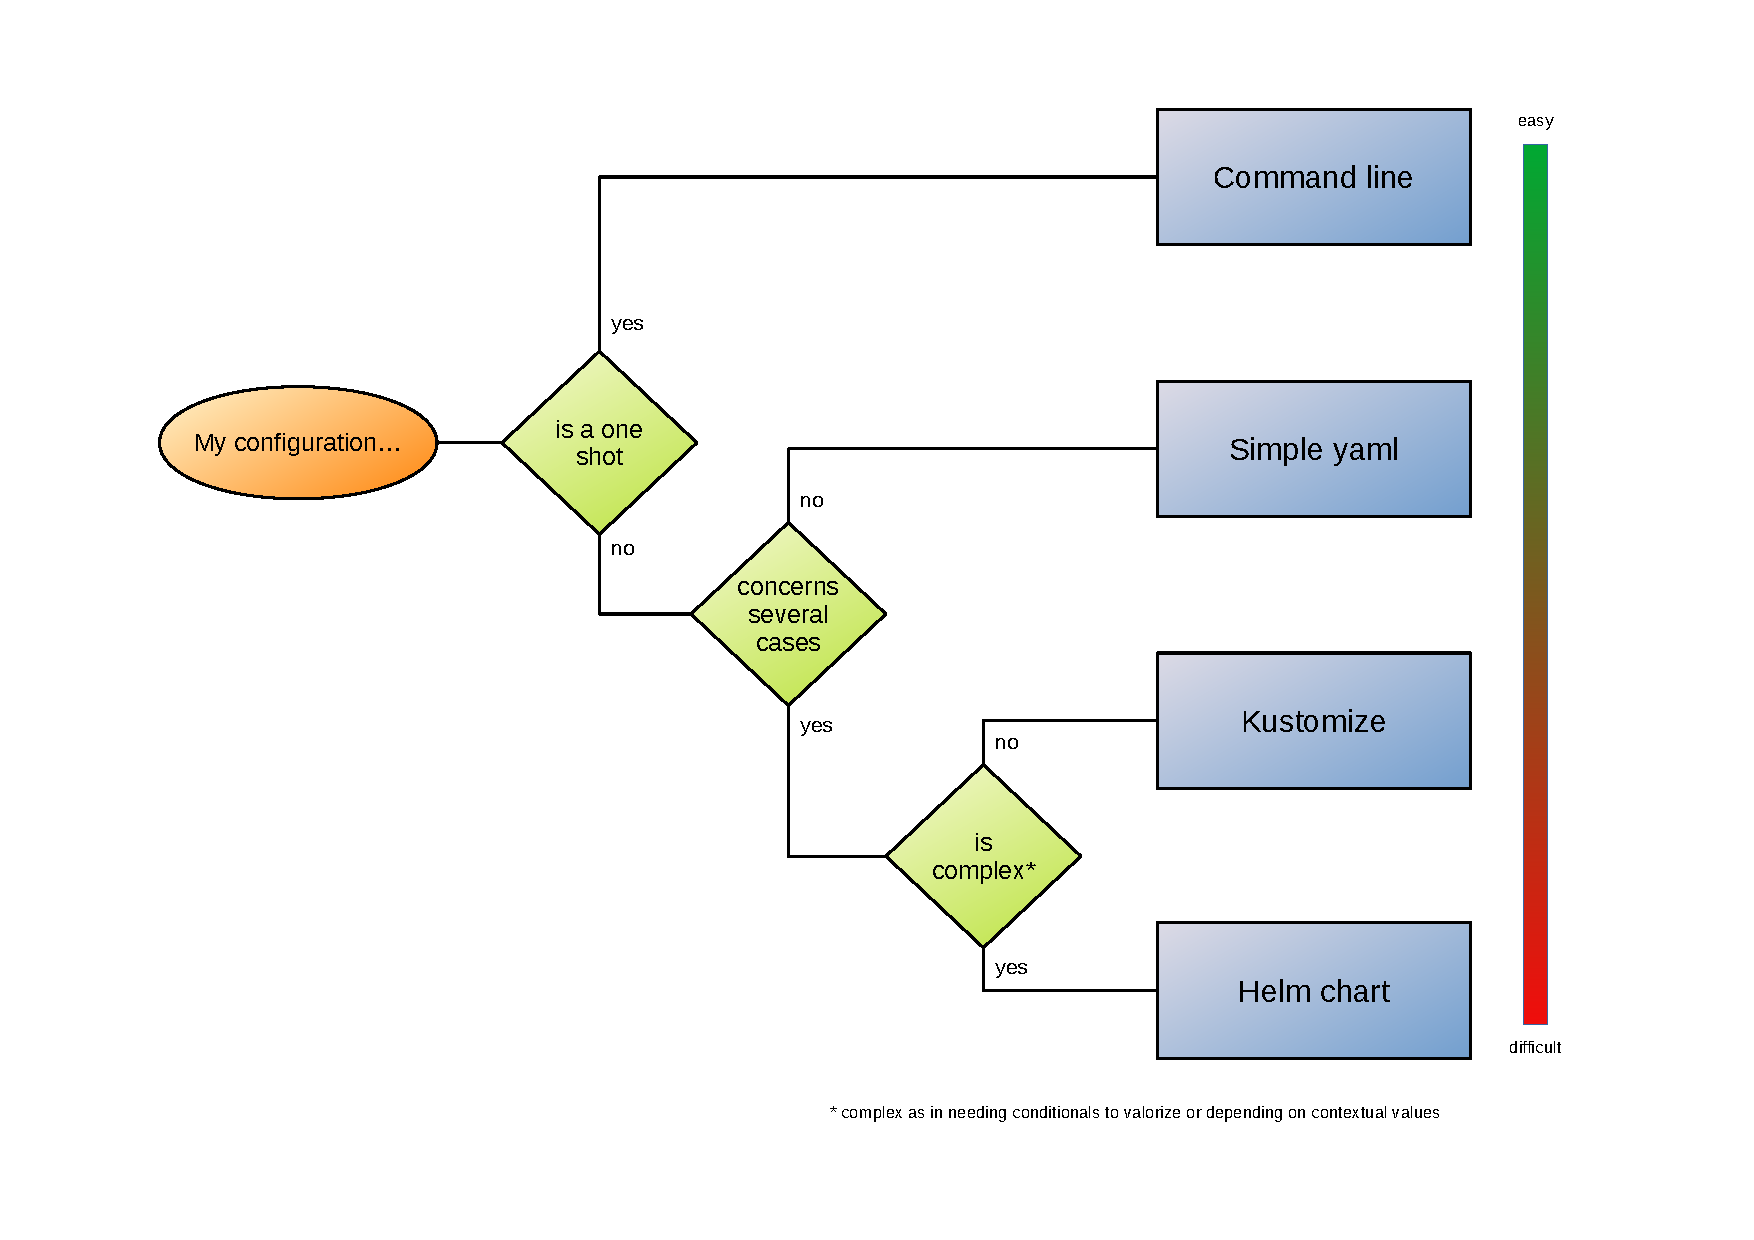
\includegraphics[height=7.5cm]{../../../resources/color/choiceConfigKind.pdf}
		\end{center}
	\end{frame}
	
	\begin{frame}
		\frametitle{Layer based configuration}
		
		Kustomize is a tool now integrated in kubectl.
		
		\bigskip
		It manage the configuration using a layer based system.
		
		That means that a configuration is the result of a base configuration, on wich layers are applyed.
		
		Eache layer can contains new resources or new patches.
		
		\bigskip
		As a base layer is considered as a resource, that enable to define a configuration as the concatenation of several other configurations and their patches.
	\end{frame}
	
	\begin{frame}[fragile]
		\frametitle{Initialize the base}
		
		We are creating a folder tree to sort our files
		\begin{block}{Command line 1}
			\begin{verbatim}
				mkdir kube
				cd kube
				mkdir base
				cd base
			\end{verbatim}
		\end{block}
	\end{frame}
	
	\begin{frame}[fragile]
		\frametitle{Initialize the base}
		
		We are starting with a fresh new deployment.yaml
		\begin{block}{source.yaml}
			\begin{tiny}
				\begin{verbatim}
						apiVersion: apps/v1
					kind: Deployment
					metadata:
					  name: worker
					  labels:
					    tinkou: worker
					spec:
					  selector:
					    matchLabels:
					      tinkou: worker
					  template:
					    metadata:
					      labels:
					        tinkou: worker
					    spec:
					      containers:
					      - name: worker
					        image: <registry>/training/worker-<id>:v1
					      imagePullSecrets:
					      - name: regcred
				\end{verbatim}
			\end{tiny}
		\end{block}
	\end{frame}
	
	\begin{frame}[fragile]
		\frametitle{Initialize the base}
		\begin{block}{Command line 1}
			\begin{verbatim}
				touch kustomization.yaml
				kustomize edit fix
				kustomize edit add resource source.yaml
				kustomize build
				kubectl apply -k .
			\end{verbatim}
		\end{block}
	\end{frame}
	
	\begin{frame}[fragile]
		\frametitle{Initialize the base}
		As we modify an immutable field, we need to delete the previous deployment before:
		\begin{block}{Command line 1}
			\begin{verbatim}
				kubectl delete deployment worker
				kubectl apply -k .
			\end{verbatim}
		\end{block}
	\end{frame}
	
	\begin{frame}[fragile]
		\frametitle{Add a parameter to our worker}
		
		Modify the worker to use a parameter:
		\begin{block}{worker.sh}
			\begin{verbatim}
				while true; do
				  echo "I'm $NAME and it is $(date)"
				  sleep 2
				done
			\end{verbatim}
		\end{block}
	\end{frame}
	
	\begin{frame}[fragile]
		\frametitle{Deploy the new version in our cluster}
		
		First we need to create a new version of the image:
		\begin{block}{Command line 1}
			\begin{verbatim}
				docker build -t <registry>/training/worker-<id>:v2 \
				                ../../
				docker push <registry>/training/worker-<id>:v2
			\end{verbatim}
		\end{block}
	\end{frame}
	
	\begin{frame}[fragile]
		\frametitle{Deploy the new version in our cluster}
		
		Change the deployment configuration:
		\begin{block}{source.yaml}
			\begin{small}
				Replace v1 by v2
			
				Add to the containers spec part:
				\begin{verbatim}
					spec:
					  containers:
					    env:
					    - name: NAME
					      value: <myName>
				\end{verbatim}
			\end{small}
		\end{block}
		
		And finaly apply the modification:
		\begin{block}{Command line 1}
			\begin{small}
					\begin{verbatim}
					kubectl apply -k .
				\end{verbatim}
			\end{small}
		\end{block}
	\end{frame}
	
	\begin{frame}
		\frametitle{Deploy the new version in our cluster}
		
		There are too many operations.
		
		\bigskip
		Is there a way to simplify this?
	\end{frame}
	
\subsection{Use skaffold}	
	
	\begin{frame}
		\frametitle{Skaffold}
		
		Skaffold is a developper oriented tool create to simplify the packaging and deployment on kubernetes.
		
		\medskip
		The Skaffold documentation can be found \href{https://github.com/GoogleContainerTools/skaffold}{her}.
		
		\medskip
		Installation documentation can be found \href{https://skaffold.dev/docs/getting-started}{here}.
	\end{frame}
	
	\begin{frame}[fragile]
		\frametitle{Initialize skaffold}
		
		Let's return in WORKER\_DIR and initialize skaffold:
		\begin{block}{Command line 1}
			\begin{verbatim}
				skaffold init
			\end{verbatim}
			Follow the application command line interface.
		\end{block}
	\end{frame}
	
	\begin{frame}[fragile]
		\frametitle{Initialize skaffold}

		By default skaffold detect the yaml, so it need to be configured to use kustomize:
		\begin{block}{skaffold.yaml}
			Remove the tag from the image
			
			\medskip
			Replace the block .deploy.kubectl by:
			\begin{verbatim}
				deploy:
				  kustomize:
				    path: kube/base			
			\end{verbatim}						
		\end{block}
	\end{frame}
	
	\begin{frame}[fragile]
		\frametitle{Using skaffold}
		
		We are going to test a little skaffold commands:
		\begin{block}{Command line 1}
			\begin{verbatim}
				skaffold build
				skaffold run
				skaffold delete
				skaffold dev
			\end{verbatim}					
		\end{block}
		
		Try to modify the file worker.sh.
	
	\end{frame}
	
	\begin{frame}[fragile]
		\frametitle{Create a kustomize layer for skaffold}
		
		Skaffold do not upgrade the image…
		\begin{block}{Command line 4}
			\begin{verbatim}
				kubectl describe deployment worker
			\end{verbatim}
		\end{block}
		
	\end{frame}
	
	\begin{frame}[fragile]
		\frametitle{Create a kustomize layer for skaffold}
		We need to let skaffold manage the image tag version, by created a dedicated configuration:
		\begin{block}{Command line 4}
			\begin{small}
				\begin{verbatim}
					cd kube
					mkdir skaffold
					vi patch.yaml
				\end{verbatim}
			\end{small}
		\end{block}
		
		\begin{block}{patch.yaml}
			\begin{tiny}
				\begin{verbatim}
					apiVersion: apps/v1
					kind: Deployment
					metadata:
					  name: worker
					spec:
					  template:
					    spec:
					      containers:
					      - name: worker
					        image: <registry>/training/worker-<id>
				\end{verbatim}
			\end{tiny}
		\end{block}
	\end{frame}
	
	\begin{frame}[fragile]
		\frametitle{Create a kustomize layer for skaffold}

		\begin{block}{Command line 4}
			\begin{verbatim}
				touch kustomization.yaml
				kustomize edit fix
				kustomize edit add resource ../base
				kustomize edit add patch patch.yaml
			\end{verbatim}
		\end{block}
		Indicate the new kustomize source to skaffold:
		\begin{block}{skaffold.yaml}
			\begin{verbatim}
				deploy:
				  kustomize:
				    path: kube/skaffold
			\end{verbatim}
		\end{block}
		And the worker should be automatically updated.
		
	\end{frame}
	
	\begin{frame}[fragile]
		\frametitle{Isolate the configuration in a configmap}

		Add a file conf.env in the folder base:
		\begin{block}{conf.env}
			\begin{verbatim}
				NAME=Georges
			\end{verbatim}
		\end{block}				
		
		\begin{block}{Command line 4}
			\begin{verbatim}
				kustomize edit add configmap worker \
				                   --from-env-file conf.env
			\end{verbatim}
		\end{block}
		
		\begin{block}{source.yaml}
			Replace the block .spec.template.spec.containers.env by:
			\begin{verbatim}
				envFrom:
				  - configMapRef:
				      name: worker
			\end{verbatim}
		\end{block}
	\end{frame}
	
	\begin{frame}[fragile]
		\frametitle{Define a dev configuration}
		
		Create a configuration specific to the current development:
		\begin{block}{patch.yaml}
			Add a the file end:
			\begin{verbatim}
				---
				apiVersion: v1
				kind: ConfigMap
				metadata:
				  name: worker
				data:
				  NAME: Marion
			\end{verbatim}
		\end{block}
	\end{frame}
	
	\begin{frame}[fragile]
		\frametitle{Skaffold dev modification detection}
		
		Try to modify (or just touch) several files to test which one trigger a skaffold build or run.
		
		And finally clean everything with Ctrl+C to interrupt the skaffold dev command.
	\end{frame}
	
	\section{Batch and scheduling}

\subsection{Objectives}

	\begin{frame}
		\frametitle{Objectives}
		
		Our worker is fine, but induces too much stress on the system.We now want to deploy it as a batch.
		
		\bigskip
		As such, we want to be able to schedule it.
		
		\bigskip
		We are now going to create a batch performing the same task as our worker.
	\end{frame}

	\begin{frame}
		\frametitle{What kind to use to deploy our application}
		
		\begin{center}
		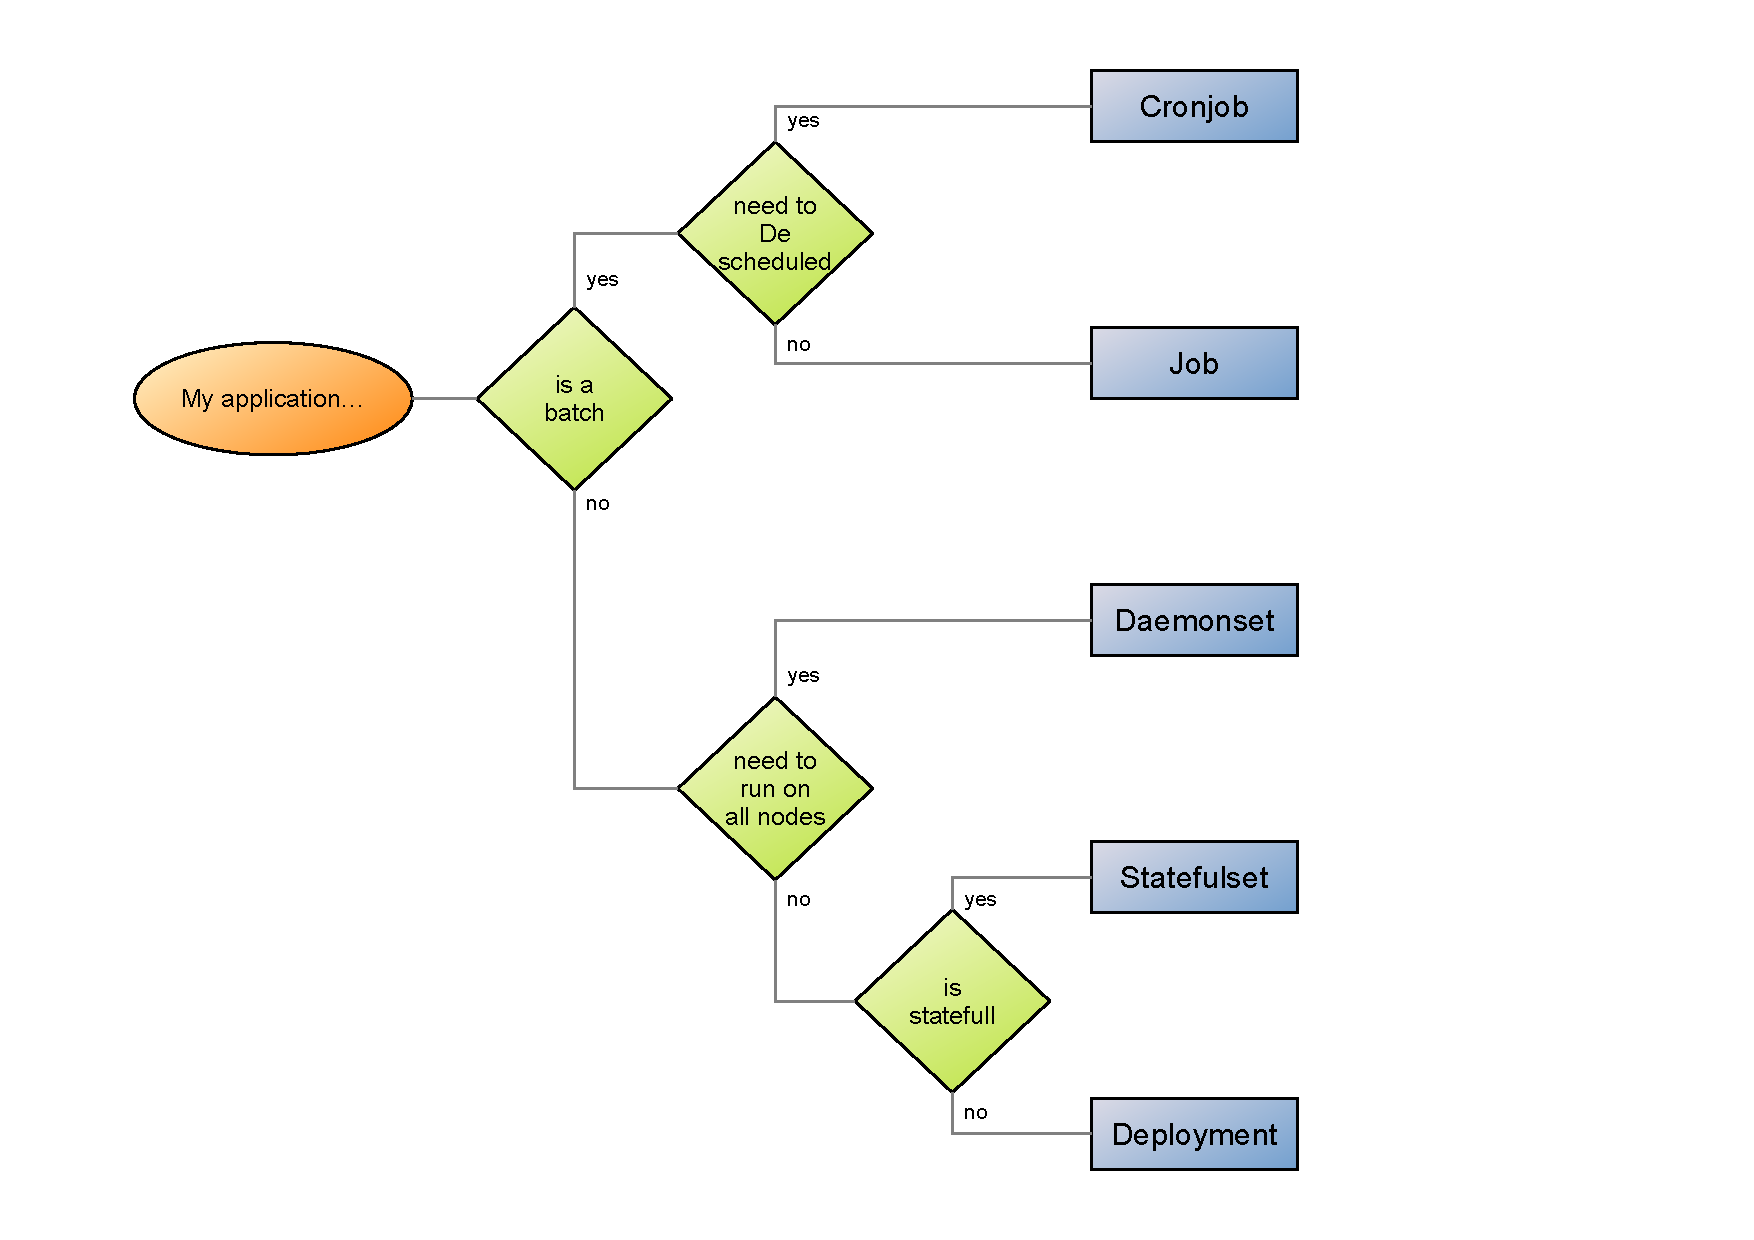
\includegraphics[height=6.8cm]{../../../resources/color/choiceDeploymentType.pdf}
		\end{center}
	\end{frame}
		
\subsection{Creating a batch in kubernetes}		
		
	\begin{frame}[fragile]
		\frametitle{Creating the batch}
		
		Beside the folder \verb!worker!, create a folder \verb!batch!.
		
		\bigskip
		Create the batch itself:
		\begin{block}{\href{https://github.com/Tinkou/trainings/blob/master/trainings/sources/dev-onboarding/files/batch/batch.sh}{batch/batch.sh}}
			\begin{verbatim}
				echo "I'm Humphrey and it is $(date)"
			\end{verbatim}
		\end{block}
		Now, each execution is unitary.
	\end{frame}
	
	\begin{frame}[fragile]
		\frametitle{Exercise}
		
		Build and run in docker an image \verb|tinkou/batch:v1| containing this batch.
	\end{frame}

	\begin{frame}[fragile]
		\frametitle{A solution}
		
		\begin{block}{\href{https://github.com/Tinkou/trainings/blob/master/trainings/sources/dev-onboarding/files/batch/Dockerfile}{batch/Dockerfile}}
			\begin{verbatim}
				FROM alpine
				
				COPY batch.sh .
				RUN chmod u+x batch.sh
				
				CMD /batch.sh
			\end{verbatim}
		\end{block}
		
		\begin{block}{Command terminal in folder batch}
			\begin{verbatim}
				docker build -t tinkou/batch:v1 .
				docker run tinkou/batch:v1
			\end{verbatim}
		\end{block}
	\end{frame}
				
	\begin{frame}[fragile]
		\frametitle{Creating our first CronJob}
		
		\begin{block}{\href{https://github.com/Tinkou/trainings/blob/master/trainings/sources/dev-onboarding/files/batch/cronjob.yaml}{batch/cronjob.yaml}}
			\begin{tiny}
				\begin{verbatim}
					apiVersion: batch/v1beta1
					kind: CronJob
					metadata:
					  name: my-batch
					spec:
					  schedule: "* * * * *"
					  jobTemplate:
					    spec:
					      template:
					        metadata:
					          labels:
					            tinkou: batch
					        spec:
					          containers:
					          - name: runner
					            image: tinkou/batch:v1
					          restartPolicy: Never
				\end{verbatim}
			\end{tiny}
		\end{block}
	\end{frame}
	
	\begin{frame}[fragile]
		\frametitle{Creating our first CronJob}
		
		\begin{block}{Logs terminal}
			\begin{verbatim}
				stern -l tinkou=batch
			\end{verbatim}
		\end{block}
		
		\begin{block}{Monitor terminal}
			\begin{verbatim}
				watch kubectl get all
			\end{verbatim}
		\end{block}
		
		\begin{block}{Command terminal}
			\begin{verbatim}
				kubectl apply -f cronjob.yaml
			\end{verbatim}
			Wait for a few batches to run…
			\begin{verbatim}
				kubectl logs -l tinkou=batch
			\end{verbatim}
		\end{block}
	\end{frame}

	\begin{frame}
		\frametitle{Creating our first CronJob}
		
		\begin{block}{Conclusions}
			\begin{itemize}
				\item[$\bullet$] CronJob are easy to defined
				\item[$\bullet$] stern is less adapted than a standard kubectl logs for jobs
			\end{itemize}
		\end{block}
		
		\begin{block}{CronJobs useful options}
			\begin{itemize}
				\item[$\bullet$] A field .spec.suspend suspend the scheduling of a CronJob
				\item[$\bullet$] Jobs in error aren't removed
				\item[$\bullet$] The history limit of successful jobs can be set
			\end{itemize}
		
		\end{block}
	\end{frame}
	
\subsection{Using a layer based configuration}	
	
	\begin{frame}
		\frametitle{Exercise}
		
		Modify the configuration to use kustomize and skaffold with:
		\begin{itemize}
			\item[$\bullet$] a base configuration similar as the current one
			\item[$\bullet$] a local configuration for minikube with NAME=Dolph
		\end{itemize}
	\end{frame}
	
	\begin{frame}[fragile]
		\frametitle{A solution}
		
		\begin{block}{Folder tree in batch folder}
			\begin{small}
				\begin{verbatim}
					batch
					|- batch.sh
					|- Dockerfile
					|- kube
					   |- base
					   |  |- conf.env
					   |  |- cronjob.yaml
					   |  |- kustomization.yaml
					   |- local
					      |- conf.yaml
					      |- kustomization.yaml
				\end{verbatim}
			\end{small}
		\end{block}

		\begin{block}{batch/kube/base/conf.env}
			\begin{small}
				\begin{verbatim}
					NAME=Humphrey
				\end{verbatim}
			\end{small}
		\end{block}

	\end{frame}
	
	\begin{frame}[fragile]
		\frametitle{A solution}
				
		\begin{block}{batch/kube/base/cronjob.yaml}
			\begin{tiny}
				\begin{verbatim}
					apiVersion: batch/v1beta1
					kind: CronJob
					metadata:
					  name: my-batch
					spec:
					  schedule: "* * * * *"
					  jobTemplate:
					    spec:
					      template:
					        metadata:
					          labels:
					            tinkou: batch
					        spec:
					          containers:
					          - name: runner
					            image: tinkou/batch:v1
					            envFrom:
					            - configMapRef:
					                name: batch
					          restartPolicy: Never
				\end{verbatim}
			\end{tiny}
		\end{block}
	\end{frame}
	
	\begin{frame}[fragile]
		\frametitle{A solution}

		\begin{block}{Command terminal in folder batch/kube/base}
			\begin{verbatim}
				kustomize create --resources cronjob.yaml
				kustomize edit add configmap batch \
				                             --from-env-file conf.env
			\end{verbatim}
		\end{block}
	\end{frame}
	
	\begin{frame}[fragile]
		\frametitle{A solution}
		
		\begin{block}{batch/kube/local/conf.yaml}
			\begin{verbatim}
				apiVersion: v1
				kind: ConfigMap
				metadata:
				  name: batch
				data:
				  NAME: Dolph
			\end{verbatim}
		\end{block}
	\end{frame}
	
	\begin{frame}[fragile]
		\frametitle{A solution}
		
		\begin{block}{Command terminal in folder batch/kube/local}
			\begin{verbatim}
				kustomize create --resources ../base
				kustomize edit add patch conf.yaml
			\end{verbatim}
		\end{block}
	\end{frame}
	
	\begin{frame}[fragile]
		\frametitle{A solution}
		
		\begin{block}{batch/skaffold.yaml}
			\begin{footnotesize}
				\begin{verbatim}
					apiVersion: skaffold/v1beta12
					kind: Config
					build:
					  artifacts:
					  - image: tinkou/batch
					deploy:
					  kustomize:
					    path: kube/base
					profiles:
					- name: local
					  activation:
					  - kubeContext: minikube
					  deploy:
					    kustomize:
					      path: kube/local
				\end{verbatim}
			\end{footnotesize}
		\end{block}
	\end{frame}
	
	\begin{frame}[fragile]
		\frametitle{A solution}
		
		\begin{block}{Command terminal in folder batch}
			\begin{verbatim}
				skaffold run
			\end{verbatim}
		\end{block}
		
		\bigskip
		
		Take a quick look at the scheduling options and logs:
		\begin{block}{Command terminal}
			\begin{verbatim}
				kubectl describe cronjob my-batch
			\end{verbatim}
		\end{block}
		
		\bigskip
		
		Clean after working:
		\begin{block}{Command terminal in folder batch}
			\begin{verbatim}
				skaffold delete
			\end{verbatim}
		\end{block}
	\end{frame}
	
	\begin{frame}
		\begin{center}
			Questions?
		\end{center}
	\end{frame}
	
	\section{Web service}

	\begin{frame}
		WIP
	\end{frame}
	
\end{document}